\documentclass[11pt,letterpaper]{article}
\usepackage[T1]{fontenc}
\usepackage{lmodern,amsmath,amsthm,amssymb,mathtools}
\usepackage[margin=1.02in,top=0.88in,bottom=0.9in]{geometry}
\usepackage{xcolor,microtype,enumitem,tikz,needspace,hyperref,fancyhdr}
\definecolor{ink}{HTML}{153F53}
\definecolor{link}{HTML}{145774}
\hypersetup{colorlinks=true,linkcolor=link,urlcolor=link,citecolor=link,
pdftitle={The constructive hairy ball theorem in intuitionistic primitive recursive arithmetic},
pdfauthor={Research note}}
\pagestyle{fancy}\fancyhf{}\fancyhead[L]{\small\itshape The constructive hairy ball theorem}
\fancyhead[R]{\small iPRA}\fancyfoot[C]{\small\thepage}
\renewcommand{\headrulewidth}{0.25pt}\setlength{\headheight}{14pt}
\newtheorem{theorem}{Theorem}[section]
\newtheorem{lemma}[theorem]{Lemma}
\newtheorem{corollary}[theorem]{Corollary}
\theoremstyle{definition}\newtheorem{definition}[theorem]{Definition}
\newcommand{\Q}{\mathbb Q}\newcommand{\N}{\mathbb N}\newcommand{\Z}{\mathbb Z}
\newcommand{\R}{\mathbb R}\newcommand{\ipra}{\mathrm{iPRA}}
\newcommand{\len}[1]{\lVert #1\rVert_1}
\newcommand{\dy}[1]{2^{-#1}}\newcommand{\rad}{\operatorname{rad}}
\newcommand{\clog}{\operatorname{clog}}\newcommand{\code}[1]{\texttt{\small #1}}
\setlist[itemize]{leftmargin=*,itemsep=2pt,topsep=4pt}
\setlist[enumerate]{leftmargin=*,itemsep=3pt,topsep=4pt}
\setcounter{tocdepth}{1}
\setlength{\emergencystretch}{2em}
\raggedbottom
\begin{document}
\thispagestyle{plain}
\noindent{\sffamily\bfseries\color{ink}\fontsize{23}{27}\selectfont The constructive hairy ball theorem\par}
\vspace{3pt}
\noindent{\sffamily\large in intuitionistic primitive recursive arithmetic\par}
\vspace{12pt}
\noindent
On every even-dimensional sphere, a uniformly presented tangent field has a
small vector at an explicitly computable point. For any requested error
$2^{-k}$ we construct a point \emph{with rational coordinates on the
round sphere} at which the field has norm at most $2^{-k}$. The field
may have real values and need only come with a primitive recursive
modulus of uniform continuity. The proof reduces to one integer
coefficient. If every tested vector were too large, a sequence of finite
labelings would preserve that coefficient while changing it from $1$ to
$-1$. We also show why requiring an exact zero changes the
computational content, even for a simple family of smooth fields.
\par\vspace{6pt}\hrule\vspace{4pt}
\section{The field and the arithmetic statement}\label{sec:presentation}
Let $n=2m$, $d=n+1$, and put
\[
 S^n=\{x\in\R^d:x\cdot x=1\},\qquad
 P_{\Q}=\{p\in\Q^d:\len p=1\},\qquad
 \rad(p)=p/\sqrt{p\cdot p}.
\]
The tangent plane at $\rad(p)$ consists of the vectors $v$ with
$p\cdot v=0$. We use $\ell^1$ distance for inputs and outputs. A bound
in this norm also bounds the Euclidean norm. Using the radial parameter
keeps the triangulation rational. The vector values stay in the same
ambient coordinates throughout. The classical theorem asks for an
exact zero \cite{wiki}. Approximate-zero search for circuit inputs has
also been studied in computational complexity \cite{gh}.

Here iPRA means first-order intuitionistic arithmetic with a symbol and
defining equations for each fixed primitive recursive (PR) definition,
successor axioms, and quantifier-free induction. A theorem about a
presented field is a schema for fixed PR terms, with free number
parameters allowed. A finite table is itself a number and may be
quantified over. This is also the convention of ProveIt's embedded
object calculus \cite{deriv}. We give the numerical theorem first so the
meaning of a real-valued field is explicit.

\begin{definition}[A field name]\label{def:name}
Fix PR functions $A(p,h)\in\Q^d$ and $\mu(h)\in\N$. The following
rational inequalities are the contract on $p,q\in P_\Q$ and
$h,j\in\N$:
\begin{align}
 j\ge h\quad &\Longrightarrow\quad
       \len{A(p,j)-A(p,h)}\le 2\cdot 2^{-h},                  \tag{C}\\
 \len{p-q}\le2^{-\mu(h)}\quad &\Longrightarrow\quad
       \len{A(p,h)-A(q,h)}\le3\cdot 2^{-h},                   \tag{U}\\
 & |p\cdot A(p,h)|\le2^{-h}.                                 \tag{T}
\end{align}
Encodings are canonical at a rational input, or the evaluator is first
composed with rational reduction. There is no monotonicity assumption
on $\mu$. For each fixed $p$, the sequence $A(p,h)$ is a name of the
field value at $\rad(p)$. Condition (T) permits tangency error in each
rational reading.
\end{definition}

\begin{theorem}[A bounded witness in iPRA]\label{thm:main}
For every field name in dimension $n=2m$ there is a PR function $W$
with the following property provable in iPRA under (C), (U), (T).
Given $k\in\N$, set $t=k+6$, $D=2d\,2^{\mu(t)}$, and $q=W(k)$.
Then
\[
  q\in P_\Q,\quad Dq\in\Z^d,\quad
  \len{A(q,t)}\le\tfrac34\,2^{-k},\qquad
  \forall j\ge t\quad \len{A(q,j)}\le\tfrac{25}{32}\,2^{-k}.
\]
The search evaluates $A$ at a single precision on the signed simplex
grid of denominator $D$. A bound on the number of candidate occurrences is
$2^d\binom{D+d-1}{d-1}$. Repeated points may be scanned or omitted.
\end{theorem}

The last inequality gives a margin for interpreting the answer as a
real vector. Every ordinary tolerance $\varepsilon=u/v>0$ reduces to
a dyadic request, for example $k=v$ for positive integers $u,v$ since
$2^v\ge v$. Section~\ref{sec:round} gives the round-sphere version and
the conversion to a rational unit-vector witness. Sections~\ref{sec:table}
and~\ref{sec:finite-degree} prove the finite obstruction used in the search.
For $n=0$ one may simply take $q=1$, since (T) bounds its only component.

The starting point in ProveIt is the sphere chapter of the general
topology packet \cite{spheres}. Its results S01--S06 establish the
finite antipodal obstruction and a search for exactly tangent,
rational-valued Lipschitz fields. The chapter identifies the
real-valued evaluator as a remaining extension. The proof below
supplies that extension: it corrects a single noisy evaluation
at each proof vertex, permits a general modulus, and does not need a
global bound on the size of the field.

\section{A finite tangent-field theorem}\label{sec:table}

Put $d=n+1$. Realize the boundary of the $d$-dimensional
cross-polytope as $P=\{p:\|p\|_1=1\}$, with vertices
$+e_1,-e_1,\ldots,+e_d,-e_d$. We use only the rational vertices
of its $r$-fold barycentric subdivision, denoted here by $K_r$.
Its mesh is the largest $\ell^1$ distance between two vertices of one
simplex. The norms in this section are the rational operations
$\|a\|_1=\sum_i|a_i|$ and $\|a\|_\infty=\max_i|a_i|$.

\begin{theorem}[Finite small-vector witness]\label{thm:finite-table}
Suppose $n$ is even, $\tau>0$ is rational, and the mesh of $K_r$ is
at most $1/(8d)$. At every vertex $p$ let a rational vector $v_p$
be given, with $p\cdot v_p=0$. Assume that for every edge $[p,q]$,
\[
             \|v_p-v_q\|_1\leq \frac{\tau}{16d}.
\]
Then a bounded scan of the vertices returns a vertex $p$ with
$\|v_p\|_1\leq\tau$.
\end{theorem}

The geometry of the failed-scan argument takes place in a plane. If a
vertex value is large, rescale it to a tangent vector $w_p$ of unit
$\ell^1$ norm. Join $p$ to $w_p$, then $w_p$ to $-p$, by straight
segments. Orthogonality keeps both segments away from the origin.
The proof measures that separation uniformly over all vertices.
\begin{center}
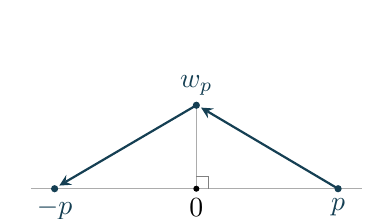
\begin{tikzpicture}[x=1cm,y=1cm,>=stealth]
  \draw[gray!65] (-2.1,0)--(2.1,0);
  \draw[gray!65] (0,0)--(0,1.03);
  \draw[gray] (0.15,0)--(0.15,.15)--(0,.15);
  \draw[ink,thick,->] (1.8,0)--(.06,1.03);
  \draw[ink,thick,->] (0,1.06)--(-1.74,.04);
  \fill[ink] (1.8,0) circle (1.3pt) node[below] {$p$};
  \fill[ink] (-1.8,0) circle (1.3pt) node[below] {$-p$};
  \fill[ink] (0,1.06) circle (1.3pt) node[above] {$w_p$};
  \fill (0,0) circle (1.1pt) node[below] {$0$};
\end{tikzpicture}
\end{center}

\begin{proof}
For $n=0$, the two directions are $p=\pm1$ and tangency forces
$v_p=0$. For $n>0$, scan the table in vertex order and return the
first entry satisfying the conclusion. The remaining branch has
$A_p=\|v_p\|_1>\tau$ at every vertex. Define $w_p=v_p/A_p$.
Then $p\cdot w_p=0$ and $\|p\|_1=\|w_p\|_1=1$. If $p,q$
are vertices of one simplex, the edge hypothesis and the reverse
triangle inequality give
\[
 \|w_p-w_q\|_1
 \leq \frac{\|v_p-v_q\|_1+|A_q-A_p|}{A_p}
 \leq \frac{2\|v_p-v_q\|_1}{\tau}
 \leq \frac1{8d}.
\]
This includes $p=q$.

Take $L=16d$. Make $2L+1$ tables $H_i$, each with one rational
vector per vertex, using the two formulas
\[
 \begin{split}
 H_j(p)&=(1-s)p+s w_p,\\
 H_{L+j}(p)&=(1-s)w_p-s p,
 \qquad s=j/L,\quad 0\leq j\leq L .
 \end{split}
\]
The two formulas agree at $H_L$. The squared length of any entry
is at least $((1-s)^2+s^2)/d$. Indeed, the cross term vanishes by
tangency, and for any $a$ of $\ell^1$ norm one the identity
\[
 d\sum_i a_i^2-\Big(\sum_i|a_i|\Big)^2
   =\sum_{i<j}(|a_i|-|a_j|)^2
\]
gives $\sum_i a_i^2\geq 1/d$. As $(1-s)^2+s^2\geq 1/2$,
and $\sum_j (H_i(p)_j)^2\leq d\|H_i(p)\|_\infty^2$, it follows
by rational comparison that
\[
                      \|H_i(p)\|_\infty\geq\frac{1}{2d}.
\]
At any one time the $\ell^1$ distance between two entries on the
same simplex is at most $1/(8d)$, by the mesh bound and the estimate
on $w_p-w_q$. At a fixed vertex one time step changes the entry by
at most $2/L$ in $\ell^1$, since each endpoint vector of each leg has
norm one. Consequently, for $p,q$ in a common simplex and
$|i-i'|\leq1$,
\[
       \|H_i(p)-H_{i'}(q)\|_\infty
        \leq \frac{1}{8d}+\frac{2}{L}=\frac{1}{4d}.
\]

Label $p$ at time $i$ by the signed basis vector corresponding to the
first coordinate of $H_i(p)$ of largest absolute value, with its
observed sign. If entries on the same simplex at equal or adjacent
times received labels $+e_j$ and $-e_j$, their $j$th coordinates
would differ by at least $1/d$. This contradicts the preceding upper
bound. A collection of signed basis vertices containing no opposite
pair spans a face of the cross-polytope. Hence the labels at each
time define a simplicial map, and maps at consecutive times are
contiguous because the union of their labels on each source simplex
spans a target face.

At time zero the label $\lambda(p)$ is the signed largest coordinate
of $p$ with the same tie convention. Its coordinate is nonzero, so
it belongs to the smallest original face containing $p$. Thus
$\lambda$ is a carrier map. At the final time the labels are
$-\lambda(p)$, because the first maximizing index is unchanged
by negation. The contiguous sequence from $\lambda$ to $-\lambda$
contradicts Theorem~\ref{thm:obstruction}. This eliminates the
unsuccessful branch of the bounded scan.
\end{proof}

The computation returning $p$ only compares the entries of the
original table with $\tau$. Normalized vectors and labels certify
why this scan succeeds. Their denominators are positive on the branch
where they are used, and the proof uses only rational arithmetic and
bounded loops.

\section{The finite obstruction on a cross-polytope}
\label{sec:finite-degree}

Write $d=n+1$. Let $K$ be the simplicial complex with vertices
$+1,-1,\ldots,+d,-d$ whose faces are the subsets containing no opposite
pair. Geometrically the signed index $\sigma i$ stands for $\sigma e_i$.
Thus $|K|=\{x\in\mathbb R^d:\sum_i|x_i|=1\}$, and every simplex used
below has rational vertices. Write $K_r$ for the $r$-fold barycentric
subdivision, with $K_0=K$. A vertex $x$ of $K_r$ has a nonempty signed
support, the signed indices of its nonzero coordinates. Put
\[
    c(x)=\operatorname{sgn}(x_i)i,\qquad
    i=\min\{j: |x_j|=\max_k |x_k|\}.
\]
In particular $c(x)$ belongs to the support of $x$.

\begin{theorem}[Finite obstruction]\label{thm:obstruction}
Suppose $d$ is odd, $r\geq0$, and $T\geq1$. At every vertex $x$ of
$K_r$ and every integer $j$ from $0$ through $T$, prescribe a label
$\ell_j(x)\in\{\pm1,\ldots,\pm d\}$, with
$\ell_0(x)=c(x)$ and $\ell_T(x)=-c(x)$. There is a simplex $s$ of
$K_r$ and a $j<T$ such that among the labels
\[
       \{\ell_j(x),\ell_{j+1}(x):x\text{ a vertex of }s\}
\]
one finds opposite signed indices. A bounded scan of the finite lists
returns $j$, $s$, two vertices and their layers witnessing this assertion.
\end{theorem}

\begin{proof}
We compare one oriented chain at the two ends of the proposed sequence.

\noindent\textit{Oriented chains.}
Use integer formal sums of oriented simplices. A tuple
$[v_0,\ldots,v_p]$ changes sign under a transposition and denotes zero
if two entries coincide. Its boundary for $p>0$ is the alternating sum
obtained by deleting one entry, and a vertex has zero boundary.
A vertex map $f$ taking each simplex into a simplex gives a chain map
$f_\#[v_0,\ldots,v_p]=[f(v_0),\ldots,f(v_p)]$. Indeed the
boundary of the tuple is obtained by deleting the same entries before
or after applying $f$. If the image has repeated entries, choose two
equal entries in positions $a<b$. All deletion terms except possibly
$a,b$ still have a repeat. The two exceptional lists differ by moving
one entry across $b-a-1$ others. Their orientation signs, combined
with their deletion signs, cancel.

For an oriented simplex $s=[v_0,\ldots,v_p]$, its oriented subdivision
$S(s)$ is the following chain. For each permutation $\pi$ of
$0,\ldots,p$ take, with coefficient $\operatorname{sgn}(\pi)$, the
flag of successive barycentres of
$\{v_{\pi(0)}\},\{v_{\pi(0)},v_{\pi(1)}\},\ldots,
\{v_{\pi(0)},\ldots,v_{\pi(p)}\}$, listed in that order. This formula
is alternating in the vertices of $s$. In its boundary, deletion of
any barycentre other than the last cancels with the flag obtained by
interchanging the two consecutive vertices added across the missing
stage. If the last vertex added was $v_i$, deletion of the last
barycentre has coefficient $(-1)^i$ times the permutation sign on
the other vertices. Hence $\partial S(s)=S(\partial s)$ for $p>0$,
and the same identity holds at $p=0$. Iterate this explicit operator
to obtain $S^r$. It sends any cycle to a cycle.

\par\smallskip\noindent\textit{What the initial labels do to subdivision.}\enspace
Every fine face inside a coarse face $s$ has all its vertices supported
on signed indices belonging to $s$. Consequently the labels $c$ on
that fine face belong to $s$. In fact
\[
                          c_\# S^r(s)=s
\]
for every oriented coarse face $s$. For a vertex the identity is
immediate. For a $p$-face with $p>0$ the left side is a $p$-chain
supported on that same face, hence an integer multiple $a s$.
The boundary identity and the assertion for the facets of $s$ give
$a\partial s=\partial s$. Comparing the coefficient of just one
facet yields $a=1$. This proves the identity by induction on $p$.

\par\smallskip\noindent\textit{The cycle distinguishing the endpoints.}\enspace
For a sign vector $\sigma=(\sigma_1,\ldots,\sigma_d)$ let
$F_\sigma=[\sigma_1 e_1,\ldots,\sigma_d e_d]$ in increasing
order of the unsigned indices. Define the top chain
\[
                    Z=\sum_{\sigma\in\{\pm1\}^d}
                           (\sigma_1\cdots\sigma_d) F_\sigma.
\]
It is a cycle. For $d\ge2$ a facet with the $i$th index missing occurs
twice with the same deletion sign and opposite coefficient. For $d=1$
the boundary of each vertex is zero. The antipodal map $A(v)=-v$
sends $F_\sigma$ to $F_{-\sigma}$. Reindexing the finite sum gives
$A_\#Z=(-1)^d Z$. The coefficient on the all-positive face of $Z$ is $1$.

\par\smallskip\noindent\textit{What adjacent layers preserve.}\enspace
Suppose the scan found no opposite pair. For each pair of consecutive
layers the union of the two label sets of a fine simplex is therefore
a face of $K$. Let $f=\ell_j$ and $g=\ell_{j+1}$, two simplicial
vertex maps. Fix a total order on the fine vertices, and on each
increasing oriented basis simplex put
\[
 P[v_0,\ldots,v_p]=\sum_{i=0}^p(-1)^i
 [f(v_0),\ldots,f(v_i),g(v_i),\ldots,g(v_p)] .
\]
Extend by integer linearity. The common-face property makes every
tuple legitimate. The identity
\[
                \partial P+P\partial=g_\#-f_\#
\]
is a finite cancellation. In summand $i$, deleting $f(v_i)$ matches
deleting $g(v_{i-1})$ in summand $i-1$ with opposite coefficient
when $i>0$. The unmatched end terms are $g_\#$ and $-f_\#$.
For a deletion $f(v_k)$ with $k<i$, its coefficient is $(-1)^{i+k}$,
opposite to the coefficient $(-1)^{k+i-1}$ in $P\partial$.
For a deletion $g(v_k)$ with $k>i$, its coefficient is
$(-1)^{i+k+1}$, opposite to $(-1)^{k+i}$ in $P\partial$.
These identities also apply when images repeat, by the alternating-tuple
rule above.

The chain $S^r(Z)$ has degree $n=d-1$. Each tuple in $P(S^r(Z))$
has $d+1$ entries belonging to a single face with at most $d$ vertices,
so this chain vanishes. Also $\partial S^r(Z)=0$. Thus consecutive
layers have exactly the same top image chain. Repeating this equality
gives $Z=c_\#S^r(Z)=(A\circ c)_\#S^r(Z)=(-1)^d Z$.
For odd $d$, the coefficient at the all-positive face would give
$1=-1$. Therefore the finite scan cannot end in failure. Its success
branch already records the required witnesses.
\end{proof}

\begin{lemma}[Mesh in the $\ell^1$ metric]\label{lem:mesh}
For $n\geq1$ the diameter of every simplex after $r=ns$ barycentric
subdivisions is at most $2^{1-s}$. For $n=0$ every diameter is zero.
\end{lemma}
\begin{proof}
A coarse face has diameter at most $2$ in the $\ell^1$ norm, since
every signed coordinate vertex has norm $1$. In a fine
simplex its barycentric vertices come from a nested family of faces.
For nonempty $B\supsetneq D$,
\[
 b_B=\frac{|D|}{|B|}b_D+
       \frac{|B|-|D|}{|B|}b_{B\setminus D}.
\]
The distance of these barycentres $b_B,b_D$ is at most
$n/(n+1)$ times the diameter of the parent simplex. Indeed the
second term uses a convex combination of vertices of that simplex,
and the same bound applies to every pair in the nested family.
For $n\geq1$, Bernoulli's inequality gives
$(1+1/n)^n\geq2$. After $r=ns$ subdivisions the diameter is at
most $2^{1-s}$. For $n=0$ the diameter is already zero.
\end{proof}

\par\smallskip\noindent\textit{The induction used by the obstruction.}\enspace
The finite assertion also has a uniform arithmetic reading with $n,r,T$
as numbers. An abstract simplex can be represented by an increasing list
of vertex identifiers, an oriented tuple by its sorted list and permutation
sign, and a chain by an array of signed integer coefficients indexed by
the enumerated faces of its degree. Store the coordinate tuple alongside
each vertex identifier. To form one subdivision, enumerate nonempty faces
of the preceding complex, assign each its average, then enumerate nested
lists of those faces; their lengths are at most $d$. For instance, from
$h$ face identifiers one may try all ordered lists of length up to $d$
over $0,\ldots,h-1$ and keep strictly nested lists. This step is a
bounded loop on explicitly given numbers, and repetition for $r$ steps
is ordinary primitive recursion. The signs in $S$, $P$ and $Z$ and all
chain sums similarly have primitive-recursive implementations. One can
use signed numerator/positive denominator arithmetic throughout.

In the carrier induction proving $c_\# S^r(s)=s$, the apparent assertion
that every coarse $p$-face satisfies the identity means the Boolean
conjunction of coefficient equalities over the already enumerated faces.
The induction on $p$ is therefore quantifier-free induction with $n,r$
as parameters. The same compilation applies to the boundary and mesh
identities at subdivision stages and to equality of the image chains at
time layers. In the sign cancellations, finite contributions of opposite
signs are paired by the explicit transposition or deletion rule just given.
Summing over the resulting pairs is bounded arithmetic, justified for
example by induction on the processed prefix of a finite list. Finally,
run the witness scan with a success flag. Its failure flag implies that
every tested pair passed the no-opposites check, whence the displayed
impossible integer equality. A case split on this one Boolean proves
success and returns the stored indices intuitionistically.

\section{From noisy values to a bounded witness}\label{sec:search}
We prove Theorem~\ref{thm:main}. In this section $e=2^{-k}$.
For $v\ge1$, write $\clog(v)$ for the smallest $j\le v$ with $2^j\ge v$.
This is a bounded integer operation. Choose the proof precision
\[
 h=k+8+2\clog(d+1),\qquad \delta=2^{-h}
       \le\frac{e}{256d(d+1)},\qquad \tau=e/2 .
\]
It is finer than the output precision $t=k+6$.

\paragraph{Correcting each observed vector.}
For a rational $p\in P_\Q$ put $a_p=A(p,h)$ and define
\[
 v_p=a_p-\frac{p\cdot a_p}{p\cdot p}\,p .
\]
Since $(\sum |p_i|)^2\le d\sum p_i^2$, the denominator is at least
$1/d$. Dotting with $p$ gives exactly zero. Condition (T) and
$\len p=1$ give the explicit correction bound $\len{v_p-a_p}\le d\delta$.
At two points within $2^{-\mu(h)}$, condition (U) now gives
\[
 \len{v_p-v_q}\le(2d+3)\delta\le e/(32d)=\tau/(16d).
\]
This step only uses the individual errors and a same-precision
comparison. In particular, the correction never amplifies a large
field value in the estimate.

\paragraph{The fine witness used in the proof.}
Take $s=1+\max(\mu(h),\clog(8d))$ and $r=ns$. By
Lemma~\ref{lem:mesh} the mesh of $K_r$ is at most
$\min(2^{-\mu(h)},1/(8d))$. The preceding bounds verify the hypotheses
of Theorem~\ref{thm:finite-table} on its vertices. Thus the finite
table supplies a $p$ with $\len{v_p}\le e/2$, whence
$\len{A(p,h)}\le e/2+d\delta$.

\paragraph{Moving to the search grid.}
Write $p_i=\sigma_i b_i$ with $\sigma_i\in\{\pm1\}$, $b_i\ge0$,
$\sum b_i=1$ (choose $+1$ for zero). Set
\[
 c_i=\lfloor Db_i\rfloor\quad(i<d),\qquad
 c_d=D-\sum_{i<d}c_i,\qquad q_i=\sigma_i c_i/D .
\]
Then $c_d\ge0$ and $q\in P_\Q$. The discrepancy in the last
coordinate is the sum of the other rounding errors before restoring
signs. Hence $\len{p-q}\le2(d-1)/D\le2^{-\mu(t)}$.
Using (C) at $p$, then (U) between $p$ and $q$, gives
\[
 \len{A(q,t)}
 \le e/2+d\delta+2\cdot2^{-t}+3\cdot2^{-t}
 \le 3e/4 .
\]
For the last comparison, $d\delta\le e/256$ and $2^{-t}=e/64$.
This proves that at least one candidate passes the rational test.
The scan returns its first passing candidate in the chosen order.
For any such candidate and every $j\ge t$, (C) gives
$\len{A(q,j)}\le 3e/4+2e/64=25e/32$.
This concludes the proof of Theorem~\ref{thm:main}.

\paragraph{Search size.}
A grid point is a choice of $d$ signs and a weak composition of $D$
into $d$ parts. The bar positions in a string of $D$ marks and $d-1$
bars encode those compositions, giving the count in the theorem.
Alternatively a scan may generate signed integer tuples in $[-D,D]^d$
and filter on $\sum|c_i|=D$. Each top facet has at most $(d!)^r$
top simplices after $r$ subdivisions, by the flag formula in
Section~\ref{sec:finite-degree}. Thus $d\,2^d(d!)^r$ bounds the
number of fine vertex occurrences used in the proof. The program
returning $W(k)$ only needs the denominator-$D$ grid. Its grid size
can grow rapidly with the input modulus.

\paragraph{An object-language induction ledger.}
For definiteness, encode $(a,b)$ by $2^a(2b+1)-1$, finite lists by
their length and a nested pairing, and integers by
$0\mapsto0$, $z>0\mapsto2z$, $-z\mapsto2z-1$. Pair decoding is
bounded by the code plus one. Use a signed numerator and a positive
denominator for rationals, reducing by a bounded gcd. Operations
have defaults on malformed codes and on division by zero.
Comparisons are made by cross multiplication. Finite products of
Boolean tests express bounded universal quantifiers.
The following are the induction predicates needed in the proof.
\begin{itemize}
\item For an oriented sum, store a coefficient for every enumerated face.
After processing $j$ terms each coefficient is its signed prefix sum.
For a cancellation involution one may collect the two occurrences by
their lesser index as a bucket; the equality of the two orders of
summation follows by a rectangular double-sum calculation on prefixes.
\item At subdivision step $i$, check the coefficient equations for all
faces on the finite lists at the current stage. Use the finite face
conjunction again for the carrier proof by face dimension. For the
diameter bound, compare all vertex pairs on all enumerated simplices.
At time step $i$, compare the top-image coefficient with the initial
coefficient. All these assertions are equations or Boolean tests of PR
terms, even when $d,r$ vary.
\item For a scan of a list of length $B$, after $j$ entries a recorded
index is in range and passes the test, or the failure flag is set and
the Boolean disjunction through $j$ is false. The update either stores
the next passing index or preserves the invariant. At termination the
exhibited good grid point rules out failure.
\end{itemize}
To collect the required instances of (C), (U), (T) into a Boolean
table, keep the field hypotheses fixed and induct on the number of
instances collected, with the prefix conjunction as the induction
formula. The tail precision $j$ in Theorem~\ref{thm:main} is arbitrary
only after the witness has been computed. There is no induction on a
field contract, no choice of a modulus from continuity, and no
universal interpreter for PR programs.

\section{Fields on the round sphere}\label{sec:round}
First consider the geometric interpretation. Suppose that $F:S^n\to\R^d$
is tangent and equipped with a PR modulus $\nu$ for $\ell^1$ distance.
Suppose its values at rational unit vectors are given to any precision
by a fixed PR rational sampler. These are data one can supply, for
example, for expressions built from rational arithmetic, bounded
reciprocals and square roots on bounded intervals. The value at a
specified precision is understood to have $\ell^1$ error at most
$2^{-h}$. A coordinatewise evaluator can meet this convention by
requesting $\clog(d)$ additional bits.

For $p,q\in P_\Q$ let $\rho=\sqrt{p\cdot p}$,
$\eta=\sqrt{q\cdot q}$. Both belong to $[1/\sqrt d,1]$.
The reverse triangle inequality bounds $|\rho-\eta|$ by $\len{p-q}$.
Subtracting $p/\rho$ and $q/\eta$ and using $\len q=1$ shows
\[
 \len{\rad(p)-\rad(q)}
 \le \left(\frac1{\rho}+\frac1{\rho\eta}\right)\len{p-q}
 \le 2d\,\len{p-q}.
\]
This explains the precision shift between the two geometries. The
construction below gives a rational unit point $R(p,a)$ within
$2^{-a}$ of $\rad(p)$. Evaluate the round sampler to precision $h+2$
at $R(p,\nu(h+2))$ to obtain $A(p,h)$. Its distance from
$F(\rad(p))$ is at most $2^{-(h+1)}$. We may take
$\mu(h)=\nu(h)+\clog(2d)$. The two evaluation errors and the modulus
give (U), common-point errors give (C), and
$p\cdot F(\rad(p))=0$ gives (T). Thus Theorem~\ref{thm:main}
produces the asserted bound on the actual field value. The last
subsection gives a formulation of this transfer entirely in arithmetic.

\subsection{A rational witness on the round sphere}\label{sec:rational-round}

Suppose the field $F$ on the Euclidean unit sphere has an $\ell^1$
modulus $\nu$, so that input distance at most $2^{-\nu(j)}$ gives
output distance at most $2^{-j}$. Apply the direction-witness result at
precision $k+1$. It gives a rational $p$ of $\ell^1$ norm one whose
unit direction $x=p/\|p\|_2$ satisfies $\|F(x)\|_1\leq2^{-(k+1)}$.
We construct a rational unit vector $z$ with $\|F(z)\|_1\leq2^{-k}$.
The construction also bounds its denominator.

Choose the first $i$ maximizing $|p_i|$, put $q=|p_i|\geq 1/d$,
and let $\sigma$ be the sign of $p_i$. For a vector $u$
indexed by the $n=d-1$ remaining coordinates, write $U=\sum_{j\ne i}u_j^2$.
The inverse stereographic chart is
\[
  \Phi(u)_j=\frac{2u_j}{1+U}\quad(j\ne i),\qquad
  \Phi(u)_i=\sigma\frac{1-U}{1+U}.
\]
The identity $4U+(1-U)^2=(1+U)^2$ proves that the output lies on
the unit sphere. If $\rho=\sqrt{p\cdot p}$, the chart parameter of
$x$ is $u_j=p_j/(\rho+q)$. Indeed $U=(\rho-q)/(\rho+q)$, and
substitution gives $\Phi(u)=x$.

Put $a=\nu(k+1)$ and
\[
   t=a+\lceil\log_2(2d(d^2+d))\rceil,\qquad M=2^t,\qquad h=1/M .
\]
Here the integer ceiling logarithm is computed by bounded search.
Bisect $[0,1]$ exactly $t$ times, comparing each midpoint squared with
$p\cdot p$. Retain the upper half if the square is smaller, and the
lower half otherwise. The upper endpoint $b$ satisfies
$\rho\leq b\leq\rho+h$. Form $p_j/(b+q)$ and round each coordinate
toward zero to the nearest multiple $v_j=m_j/M$ of $h$ in that direction.
The total change from replacing $\rho$ by $b$ is at most
\[
  \sum_{j\ne i}\frac{|p_j|(b-\rho)}{(\rho+q)(b+q)}
      \leq d^2 h .
\]
Rounding adds at most $dh$ in $\ell^1$. Set $z=\Phi(v)$.
Expanding the chart formulas gives the chord identity
\[
 \|\Phi(v)-\Phi(u)\|_2^2=
 \frac{4\|v-u\|_2^2}
      {(1+\sum_{j\ne i}v_j^2)(1+\sum_{j\ne i}u_j^2)}.
\]
Thus $\|z-x\|_1\leq 2d\|v-u\|_1\leq2d(d^2+d)h\leq 2^{-a}$,
using $\|y\|_1\leq\sqrt d\,\|y\|_2$ and $\sqrt d\leq d$.
The modulus and the triangle inequality give the claimed bound on $F(z)$.
All computed quantities use rational operations. The occurrences of
$\rho$ and $u$ identify the direction whose distance the construction
certifies. The same bounds hold for their Cauchy names by the rational
bisection enclosures.

The common denominator $M^2+\sum_{j\ne i}m_j^2$ of the displayed
chart coordinates is at most $2M^2$, since $|v_j|\leq |u_j|$ and
$\sum u_j^2\leq1$. Consequently the possible outputs at precision $k$
belong to an explicit finite grid on the round sphere.


One also obtains a rational round witness directly from the arithmetic
name of Definition~\ref{def:name}, using only its modulus $\mu$.
For $q=W(k)$ and $t=k+6$, take $z=R(q,\mu(t)+1)$ and $w=z/\len z$.
Normalization $y\mapsto y/\len y$ is $2$-Lipschitz in $\ell^1$ on
the Euclidean unit sphere: subtract the two fractions, apply the
reverse triangle inequality, and use $\len y\ge1$. It follows that
$\len{w-q}\le2^{-\mu(t)}$, with both $w,q$ rational. By (U) and (C),
for $j\ge t$ the name of the field at the rational round point $z$ obeys
\[
       \len{A(w,j)}
        \le (3/4+3/64+2/64)\,2^{-k}
        =\tfrac{53}{64}\,2^{-k}.
\]

\subsection{A first-order statement using only rational unit points}
Here is a direct arithmetic proof for a field whose only input interface
is a PR sampler $B(z,h)$ on rational vectors satisfying $z\cdot z=1$.
Give it (C), (U), (T) on that domain, with $\nu$ in place of $\mu$ and
$z$ in the tangency test. There are no real quantifiers in this
hypothesis. We construct a PR rational $z=z(k)$ such that iPRA proves
\[
 z\cdot z=1,\qquad
 \forall j\ge k+10\quad \len{B(z,j)}\le 2^{-k}.                 \tag{R}
\]
In particular the actual real vector named by $B(z,-)$ has that bound.

Let $E(a)=2(2^{a+\clog(2d(d^2+d))})^2$, the denominator bound
for $R(p,a)$ just proved. Compute a uniform value bound once. Enumerate
all rational unit points written with a common denominator
$b\le E(\nu(0))$, $1\le b$, and numerators in $[-b,b]$.
Let $M$ be $5$ plus the ceiling of the largest $\ell^1$ norm of
$B(z,0)$ in this list. The axes ensure the list is nonempty.
Every rational unit $w$ has rational parameter $w/\len w$.
Its rounding at $a=\nu(0)$ is within $2^{-\nu(0)}$ and occurs on
the list. From (U) and (C) at scale zero we obtain
$\len{B(w,j)}\le M$ for every $j$. This derives the bound from the
input data.

For each $h$ put $s_h=h+4$ and choose the monotone exponent
\[
 a_h=2+\max\!\left(\max_{i\le s_h}\nu(i),\,
                      s_h+\clog(M+1)\right).
\]
Define $R_h(p)=R(p,a_h)$ and
\[
 A(p,h)=B(R_h(p),s_h),\qquad
 \mu(h)=\nu(s_h)+2+\clog(2d).
\]
If $j\ge h$, the round inputs $R_j(p)$ and $R_h(p)$ are at distance at
most $2\,2^{-a_h}\le2^{-\nu(s_h)}$. Compare the two samples first
by round (U) at $s_h$ and then by round (C) at $R_j(p)$. The result is
at most $5\,2^{-s_h}\le 2\,2^{-h}$. For (U), our $\mu(h)$ guarantees
that the exact directions are at distance at most $2^{-\nu(s_h)}/4$;
the two roundings add at most $2\,2^{-a_h}$. Round (U) then bounds the
sample difference by $3\,2^{-s_h}$. Finally write $x=\rad(p)$.
Since $p=\rho x$, $\rho\le1$, the tangency residual is bounded by
\[
 |p\cdot A(p,h)|
 \le |R_h(p)\cdot B(R_h(p),s_h)| + 2^{-a_h} M
 \le 2^{-s_h}+2^{-a_h} M\le2^{-h}.
\]
This verifies (T). Every estimate involving $\rho$ can equivalently be
read using rational upper and lower bisection endpoints. To eliminate
such an auxiliary quantity in an inequality between rationals, establish
the inequality with error $C2^{-b}$ at each precision $b$, with $C$
given by the displayed denominator bounds. If the rational inequality
fails, choose $b$ by bounded comparison with its positive rational
gap. This proves the exact rational inequality in iPRA. For example,
$\rho\eta\ge1/d$ follows directly by squaring, and dividing in a
bisection estimate may start with the lower bound $1/d$ for each
length.

Apply Theorem~\ref{thm:main} to this $A$ and take the resulting $q$.
The point $z=R_t(q)$, $t=k+6$, is rational and satisfies $z\cdot z=1$.
Its observed value is exactly $B(z,t+4)=A(q,t)$. At every $j\ge t+4$
the bound in (R) follows by adding $2\,2^{-(t+4)}$ to
$3\,2^{-k}/4$. Its common denominator is at most $E(a_t)$. This proof
of (R) operates on number codes, with the real sphere serving as the
interpretation of the rational computations.

\section{Sharpness and exact zeros}\label{sec:sharpness}
The parity restriction is sharp. If $d$ is even, pair the coordinates and
set $J(x_1,x_2,\ldots)=(-x_2,x_1,-x_4,x_3,\ldots)$. Each pair
contributes zero to $x\cdot Jx$, and $J$ preserves the Euclidean norm.
Thus there is an explicit unit-length tangent field on every
odd-dimensional unit sphere. At the other endpoint of the dimension
range, $S^0$ has zero tangent spaces and an exact zero at either point.

The uniform-modulus formulation also applies to fields that fail to be
Lipschitz. For example on $S^2$ put
\[
       F(x)=(1+\sqrt{|x_1|})\,(e_1-x_1 x).
\]
The second factor is tangent and has $\ell^1$ norm at most $1+d$.
Its change is bounded by $(1+d)\len{x-y}$, using $|x_1|\le1$ and
$\len x\le d$. The change of the square-root factor is at most
$\sqrt{\len{x-y}}$. Consequently for $\len{x-y}\le u\le1$ the total
change is at most $3(1+d)\sqrt{u}$. This gives, for example,
$\nu(h)=2(h+\clog(3(1+d)))$. Its values are sampled by bounded bisection.
At $(0,1,0)$ the first component, along
$(s,\sqrt{1-s^2},0)$ for small $s>0$, changes from $1$ to
$(1+\sqrt{s})(1-s^2)$, while the input distance is at most $2s$.
Thus no finite Lipschitz constant suffices.

\subsection{What a uniform exact-zero procedure would decide}
Even for $S^2$, selecting an exact zero of a uniformly given field
would have a logical consequence. Let $b(0),b(1),\ldots$ be binary
with at most one $1$. Form
\[
 u=(a,c,0),\qquad a=\sum_{s\ge0}2^{-s-1}b(2s),\qquad
 c=\sum_{s\ge0}2^{-s-1}b(2s+1),
 \qquad V(x)=u-(u\cdot x)x .
\]
The first $l$ terms give each coefficient to within $2^{-l}$.
Truncating at $l=h+\clog(2(1+d))+1$ is more than enough for
$\ell^1$ error $2^{-h}$ in $V$. All fields in this family have a
common continuity modulus, since $\len u\le1$ and
$\len{V(x)-V(y)}\le(1+d)\len{x-y}$. The field is smooth as a
function of $x$.

Suppose an exact zero $x$ is supplied by a fast name. Read a rational
$v$ within $1/8$ of $|x_1|$. If $v\ge1/2$, an odd occurrence of $1$
is impossible: it would make $u$ a positive multiple of $e_2$ and
force every zero to have $x_1=0$. Thus all odd bits are zero.
If $v<1/2$, an even occurrence would make $u$ a positive multiple
of $e_1$ and force $|x_1|=1$. Thus all even bits are zero. These are
constructive implications by testing each individual bit.
The resulting disjunction is the lesser limited principle of
omniscience (LLPO) on this input.

There is already a computability obstruction for a family of PR input
terms with a number parameter. Fix a machine enumeration $\varphi_i$.
Let $b_i(2s+j)$, $j=0,1$, indicate that machine $i$ on input $i$
first halts at step $s$ with output $j$. The bounded simulation is PR.
The reported parity side would give a total computable bit $c(i)$ equal
to $\varphi_i(i)$ whenever the latter is $0$ or $1$: report $0$ when
all odd bits are zero and $1$ in the other case. A program for
$i\mapsto1-c(i)$ has an index $h$; then $c(h)=1-c(h)$. This rules
out a uniform computable exact-zero selector for this family. Each one
of these particular fields individually has a computable pole. The
argument concerns uniform selection; the following example concerns a
single instance.

\subsection{A single primitive-recursively presented field whose poles have no primitive-recursive fast names}
\label{sec:no-pr-pole}

The following separation concerns the standard computability-theoretic
interpretation of iPRA. By a PR fast name of a point we mean a
primitive-recursive rational sequence with error at most $2^{-h}$ at
input $h$. We exhibit one field on $S^2$ with a PR sampler and a linear
modulus, for which neither of its two zeros has such a name.

Enumerate unary PR programs by natural numbers, treating an ill-formed
code as the constant-zero program. A Turing interpreter can evaluate any
program in this enumeration. For program $i$ write $f_i$ for its
function and put $b_i=1-\min(1,f_i(i))$. The binary sequence $(b_i)$
is computable. If it were PR, it would equal some $f_e$ and we would
have $b_e=1-b_e$. Define the real
\[
                     \alpha=\sum_{i=0}^{\infty}b_i4^{-i-1}
                                \in[0,1/3].
\]
To recover $b_i$ from a $2^{-(2i+5)}$-approximation of $\alpha$,
multiply that approximation by $4^{i+1}$ and round to the nearest
integer. The exact scaled real equals the integer coding the first
$i+1$ base-four digits plus a tail in $[0,1/3]$. The scaled error is
at most $1/8$, so rounding recovers that integer. Its residue modulo
four is $b_i$. Thus $\alpha$ has no PR fast name.

Fix a Turing machine that prints $b_0,b_1,\ldots$ successively.
After $s$ steps, let $j_s$ be the number of emitted bits and $l_s$
the base-four prefix sum of these bits. Define
\[
 I_s=[l_s,l_s+4^{-j_s}/3],\qquad
 g(t)=\sum_{s=0}^\infty 2^{-s-1}\operatorname{clamp}_{I_s}(t),
 \qquad \operatorname{clamp}_{[a,b]}(t)=\min(b,\max(a,t)).
\]
The endpoints of $I_s$ are PR in $s$: one simulates exactly $s$ steps
of a fixed machine, recording each output bit in its configuration.
One transition and iteration for a specified number of transitions are
PR. No bound on the waiting time for the next bit enters this operation.
The intervals are nested and contain $\alpha$. Their lengths tend to
zero because the machine eventually prints each bit. The sum defining
$g$ has values in $[0,1/3]$, admits a rational approximation on rational
inputs with error at most $2^{-M}/3$ from its first $M$ terms, and is
$1$-Lipschitz since each clamp has that property. Its unique fixed
point is $\alpha$. Indeed, for $t<\alpha$ every clamp is at least $t$,
and some $I_s$ has lower endpoint strictly above $t$. The corresponding
summand in $g(t)-t$ is strictly positive. The case $t>\alpha$ follows
from the upper endpoints, and $g(\alpha)=\alpha$ holds term by term.

On $P=\{p\in\mathbb R^3:\|p\|_1=1\}$ define
\[
 t(p)=\frac{p_1p_2}{\max(1/4,p_1^2)},\quad
 u(p)=(1,g(t(p)),0),\quad
 F(p)=u(p)-\frac{p\cdot u(p)}{p\cdot p}\,p .
\]
The denominator $p\cdot p$ is at least $1/3$. We give explicit
continuity and sampling bounds to verify the presentation.
For $\delta=\|p-q\|_1$, the numerator of $t$ changes by at most
$\delta$ and its denominator by at most $2\delta$. The denominators
are at least $1/4$, so $|t(p)-t(q)|\leq36\delta$ and
$\|u(p)-u(q)\|_1\leq36\delta$. Write $a=p\cdot p$ and
$b=p\cdot u(p)$. Since $\|u(p)\|_\infty=1$, we have $|b|\leq1$,
the change of $b$ is at most $37\delta$, and the change of $a$ is
at most $2\delta$. Hence $|b/a|\leq3$ and the change of $b/a$ is
at most $(3\cdot37+9\cdot2)\delta=129\delta$. Substituting into
$F$ gives $\|F(p)-F(q)\|_1\leq168\delta$.

For $A(p,h)$ evaluate the displayed rational formula at rational
$p$, using the first $M=h+1$ terms of $g$. The projection
$v\mapsto v-(p\cdot v)p/(p\cdot p)$ has $\ell^1$ operator norm
at most $4$, so the sampler error is at most $4\cdot2^{-(h+1)}/3
\leq 2^{-h}$. Its dot product with $p$ vanishes exactly. Two such
sample errors give the coherence bound, and the Lipschitz constant
$168\leq 2^8$ gives the sampled continuity bound with $\mu(h)=h+8$.
The arithmetic verification can also be made directly on truncations:
their ranges are in $[0,1/3]$, each has Lipschitz constant at most one,
and the difference of a longer and a shorter truncation is bounded by
the omitted geometric tail. These finite checks require no proof in
iPRA that the printing machine eventually emits every digit. Its
eventual progress is used in the external argument identifying the poles.

If $F(p)=0$ then $p$ and $u(p)$ are parallel. Since the first
coordinate of $u(p)$ is $1$, we have $p_1\ne0$,
$p_3=0$, $p_2/p_1=g(t(p))$ and $|p_1|=1/(1+g(t(p)))\geq3/4$.
The denominator in $t(p)$ is then $p_1^2$, proving
$t(p)=p_2/p_1=g(t(p))$. Consequently $t(p)=\alpha$.
Conversely the two poles
$\pm(1,\alpha,0)/(1+\alpha)$ satisfy $F(p)=0$.
A PR fast name of either pole gives one of $t(p)$ by the displayed
rational formula: on the coordinate cube $[-1,1]^3$ the same
$36$-Lipschitz estimate applies, and rational approximations can first
be clipped to the cube. This contradicts the decoding argument.

On the round sphere use the tangent field $x\mapsto F(x/\|x\|_1)$.
The radial map is $2$-Lipschitz in $\ell^1$ there, since
$\|x\|_1\geq1$. It carries a PR-named zero on the round sphere to a
PR-named zero on $P$. The two poles do have ordinary computable names,
since the bit-printing program eventually evaluates every digit.
The separation is precisely between PR finite-precision witnesses
and a PR fast name for an exact zero of this one field.


\section{Lean formalization and verification}\label{sec:lean}
Two standalone files build with Lean 4.19.0 and its standard library.
They give both a concrete field interface and a checked part of the
degree argument. The mathematical proof in the preceding sections
covers all even dimensions. The full object-theory derivation is a
remaining formalization task.

\paragraph{The two implemented layers.}
In \code{NamedField.lean}, a vector is
\code{Fin d} indexed with exact rational components.
The file defines the norms, distance, dot product, projection,
predicates (C), (U), (T), denominator $D$ (function \code{gridDen}),
the filtered integer grid, and the actual search
\code{firstWitness}. Its \code{GridHit} states that an accepted point
occurs on that grid. Its \code{TailBound} is the implication from an
accepted reading and (C) to the $25/32$ tail estimate.
The theorems \code{witness\_onBoundary} and \code{witness\_accepted}
extract verified properties of a returned point. The theorem
\code{assemble} proves the complete search statement conditional on
\code{GridHit} and \code{TailBound}. The file defines these two
obligations as propositions.

In \code{HairyBall.lean}, \code{finite\_obstruction} extracts a bounded
hit from unequal endpoint coefficients and preservation on the failure
branch. Its auxiliary index scan examines indices in descending order;
either enumeration order gives a good index. The theorem
\code{antipodal\_facet\_sign} proves the factor $(-1)^d$ by list
induction in arbitrary dimension. The namespace \code{Octahedron}
contains a more explicit verification for $S^2$. Its signed triangle
cochain \code{top} picks out the all-positive facet. For all $6^4$
ordered label quadruples the kernel verifies that its coboundary
vanishes when the quadruple contains no opposite pair.
\code{triangle\_prism} combines three such identities. Then
\code{chain\_prism} sums over any finite weighted triangular source,
and \code{degree\_step} gives equality of endpoint counts when the side
cochain vanishes on its boundary. \code{base\_cycle\_closed},
\code{base\_identity} and \code{base\_antipode} verify the boundary
and both counts for the eight original facets. These are ordinary Lean
theorems; the supplied files contain no admitted proofs.

\paragraph{Completing the argument in Lean.}
The following order puts a definite, testable statement at every interface.
\begin{enumerate}
\item \emph{Finite oriented chains.} Represent a complex by a duplicate-free
list of faces on ordered vertices, closed under subfaces. Implement
$\operatorname{orient}(u)$ as zero on duplicate tuples, else as the
parity of the inversion count times the increasing basis tuple.
Represent each degree's chain by a list of integer coefficients. Give
\code{boundary}, \code{push}, and \code{subdivide} the deletion,
pointwise-map and flag formulas of Section~\ref{sec:finite-degree}.
Prove $\partial f_\#=f_\#\partial$ by the two-deletion argument, and
$\partial S=S\partial$ by the explicit flag swap. A terminating
induction on the number of uncollected terms proves the signed-sum
pairing lemma. Use it for the boundary of $Z$ as well.
\item \emph{Degree obstruction.} Store the support map sending each fine
vertex to its original signed support. Prove the support and mesh bounds
when taking a rational barycentre. For a coarse $p$-face, prove
$c_\# S^r(s)=s$ by induction on its dimension, comparing a facet
coefficient. Implement the ordered prism formula with source tuples in
one global order. Prove the three deletion identities for the prism
operator, and that $d+1$ labels in a single cross-polytope face yield
zero. Applying these identities to $S^rZ$ gives the preservation
argument required by \code{finite\_obstruction}. In dimension two
\code{degree\_step} supplies the local-to-global step once the
subdivided source cycle is built.
\item \emph{Rational estimates.} Prove the triangle and reverse triangle
inequalities for \code{l1} by induction over the coordinate fold.
The identity $d\sum a_i^2-(\sum |a_i|)^2=\sum_{i<j}(|a_i|-|a_j|)^2$
follows by expansion or by adding the last coordinate. Use
cross multiplication with positive denominators to prove the projection
and normalized-edge bounds. Define the least-max label by folding over
indices, replacing only on strict improvement. The pair of inequalities
$1/(4d)<1/d$ and the signed-coordinate lower bound prove contiguity for
the two legs. In particular these proofs can run without a library of
real topology.
\item \emph{Completing the two named-field obligations.} Instantiate the
degree result on the $r$-fold subdivision in Section~\ref{sec:search}.
The projection gives exact tangency, and (T) controls its error.
Implement $\operatorname{round}_D$ by integer floor and prove its
distance bound by summing the rounding remainders. Prove membership in
\code{integerRows} by induction on the vector length, then apply the
filter lemma to the rounded vector. The displayed $3e/4$ bound now
proves \code{GridHit}. The coordinate triangle inequality and (C) give
\code{TailBound}. Apply \code{assemble}. For the round statement (R),
implement bisection by iterating the interval update and maintain
$l^2\le p\cdot p\le b^2$ and $b-l=2^{-j}$. The squared chord identity
and the integer chart formula yield the denominator and rounding bounds.
\item \emph{Embedding in the requested object theory.} Replace lists and
coefficient arrays by the pair/list codes in Section~\ref{sec:search},
rational comparisons by the corresponding PR Boolean terms, and each
fold by the equations of its fixed PR recursion. Use the repository's
\code{Core.Basic} induction and instantiation rules in
\code{IPRADerivations} \cite{deriv}. For example set
\[
 \mathsf{TabOK}(d,r,V,\tau)=
 \mathsf{MeshOK}(d,r)\ \mathbin{\wedge_B}\
 \mathsf{AllVerticesTangent}(d,r,V)\ \mathbin{\wedge_B}\
 \mathsf{AllEdgesSmall}(d,r,V,\tau).
 \]
Here the three factors respectively fold the rational tests
$\len{p-q}\le1/(8d)$ on simplex pairs, $p\cdot V[p]=0$ on
vertices, and $\len{V[p]-V[q]}\le\tau/(16d)$ on edges;
include type, shape and positivity guards at input. The closed numerical
endpoint asserts, for $d=2m+1$, that $\mathsf{TabOK}=1$ implies that
the scan index is in range and its norm test is true. Derive it by the
prefix invariants already given. For the main schema, specialize the
PR symbols for $A,\mu$, derive the finite table guard from the three
universally closed hypotheses, and instantiate the endpoint. Close the
resulting sentence in \code{Prf PRAAx []}. The existing bridge can
transport that derivation to Foundation's standard presentation. A
host-level Lean theorem about rational lists and the object derivation
are separate deliverables in this plan.
\end{enumerate}

ProveIt's \code{SphereBlueprint.lean} already defines signed vertices,
cross faces, the fundamental coefficient and its antipodal sign.
Its \code{SubdivisionNetTarget} and \code{BoundedApproximateZeroTarget}
are named obligations. It is possible to reuse the sign theorems when
porting the present proof to the repository toolchain \cite{spheres}.
The standalone files avoid a dependency on that checkout.

\Needspace{16\baselineskip}
\paragraph{A reproducible numerical example.}
The script \code{hairy\_ball.py} projects $b=(1,2,4)$ onto the plane
normal to the input direction. On the grid $D=16$ with requested
$\ell^1$ tolerance $2/5$, it returns
\[
 p=(-2,-5,-9)/16,\qquad V(p)=(7,-10,4)/55,\qquad
 \len{V(p)}=21/55<2/5.
\]
Here the dot product vanishes because $-14+50-36=0$. The exact polar
directions of this example have denominator $7$ in $P_\Q$, so the
positive residual at denominator $16$ is genuine. The degree demonstration
on that same grid uses $1{,}026$ vertices and $2{,}048$ oriented
triangles. With eight steps per leg the signed count drops from $1$
to $0$ between layers $6$ and $7$, and from $0$ to $-1$ between layers
$9$ and $10$. At the first drop the program exhibits a tetrahedron with
labels $(+2,+2,-2,-1)$. Thus one can see where the no-opposites condition
fails when normalizing near a zero on this coarse grid. The separate script
\code{round\_witness.py} implements rational stereographic rounding
and checks the distance to the true unit direction by exact comparisons
of quadratic radicals. Reproduction commands are in the archive README.

\begin{thebibliography}{9}
\bibitem{spheres} V. Reshetnikov, \emph{ProveIt}, general topology iPRA packet,
sphere chapter, results S01--S08. Snapshot
\texttt{022dfb4c54c2}.
\href{https://github.com/VladimirReshetnikov/ProveIt/blob/022dfb4c54c22782f927a903f25bcf6491b7eba2/Logic/PrimitiveRecursiveArithmetic/docs/proofs/topology/general_topology_ipra_2026-11-19/paper/sections/07_spheres.tex}{Chapter source};
\href{https://github.com/VladimirReshetnikov/ProveIt/blob/022dfb4c54c22782f927a903f25bcf6491b7eba2/Logic/PrimitiveRecursiveArithmetic/docs/proofs/topology/general_topology_ipra_2026-11-19/lean/SphereBlueprint.lean}{\texttt{SphereBlueprint.lean}}.
\bibitem{deriv} V. Reshetnikov, \emph{ProveIt}, primitive recursive
arithmetic at the same snapshot.
\href{https://github.com/VladimirReshetnikov/ProveIt/blob/022dfb4c54c22782f927a903f25bcf6491b7eba2/Logic/PrimitiveRecursiveArithmetic/Derivations/README.md}{Embedded iPRA derivations};
\href{https://github.com/VladimirReshetnikov/ProveIt/blob/022dfb4c54c22782f927a903f25bcf6491b7eba2/Logic/PrimitiveRecursiveArithmetic/Bridge/README.md}{Foundation--ConciseIPRA bridge}.
\bibitem{gh} P. W. Goldberg and A. Hollender,
\emph{The Hairy Ball Problem is PPAD-Complete}, ICALP 2019,
65:1--65:14. The authors study approximate and exact search in a
circuit model.
\href{https://doi.org/10.4230/LIPIcs.ICALP.2019.65}{doi:10.4230/LIPIcs.ICALP.2019.65}.
\bibitem{wiki} \emph{Hairy ball theorem}, article identified in the
question, for the classical statement and dimension convention.
\href{https://en.wikipedia.org/wiki/Hairy_ball_theorem}{Wikipedia}.
\end{thebibliography}

\end{document}
